% Asal-usul (tidak pernah dicetak): lihat sources/outline_sources.md (Tahun 1: sirkulasi yang digerakkan angin, giral, transpor dan upwelling Ekman, arus batas barat, sirkulasi meridional pembalikan dan massa air). Nilai soal dan latihan dari kalkulator skrip Buku 3 calc/ch29.py; gambar dari figdata/bachelor-1/ekman_hodograph.py (solusi Ekman dengan konstanta Ekman) dan stommel_gyre.py (model Stommel 1948, parameter latihan), peta dunia dari figdata/shared/geo.py.
% Fisika memiliki gaya Coriolis (diingat kembali). Buku 1 (kelas 8) memberi arus permukaan dan giral dengan kata-kata, Buku 2 (kelas 10) upwelling: di sini dibangun ulang dengan keseimbangan Ekman. Bab 26 memiliki diagram T-S dan massa air, bab 28 parameter Coriolis, angin geostrofik dan fungsi arus meridional rerata. Keseimbangan Sverdrup, argumen vortisitas dan penurunan spiral Ekman adalah volume Tahun 3; ENSO adalah volume Tahun 2.
\chapter{Sirkulasi samudra}\label{ch:b1:ocean-circulation}

Pada 1992, saat badai di Pasifik Utara, sebuah peti kemas terlepas dari kapal yang berlayar dari Hong Kong ke Amerika Serikat. Ia pecah dan melepaskan sekitar \num{29000} bebek karet dan mainan mandi lainnya, yang mengapung menjauh dan berlayar jauh dan luas; lokasi-lokasi tempat sebagian di antaranya kemudian ditemukan membantu para ilmuwan memahami arus yang telah membawanya. Mainan terapung mengikuti air permukaan, dan air permukaan samudra tidak mengembara secara acak: ia berputar dalam \omterm{def:b1:ocean-circulation:gyre}{gyre} seluas cekungan, berpacu ke utara dalam arus sempit di sepanjang pantai barat samudra, dan naik atau turun di beberapa tempat terpilih. Bab ini menjelaskan bagaimana angin menggerakkan lapisan atas samudra, mengapa air bergerak tegak lurus terhadap angin yang mendorongnya, mengapa arus terkuat menempel pada sisi barat samudra, dan bagaimana pembalikan lambat membawa air ke jurang dan kembali.
% ledger: noaa:floatees

\begin{omfigure}
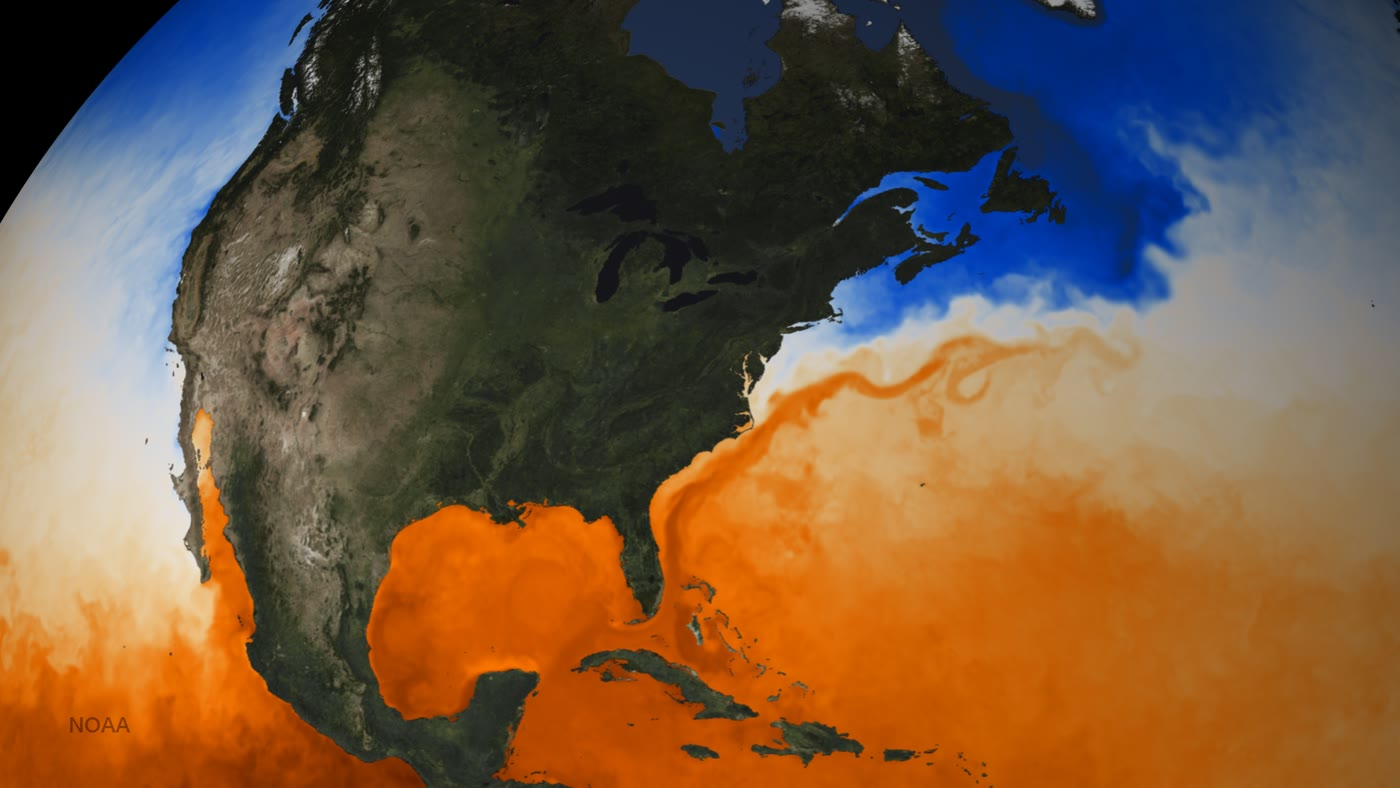
\includegraphics[width=0.85\linewidth]{images/book3/b1-gulf-stream-sst.jpg}

{\small Suhu permukaan laut di sekitar Amerika Utara pada awal Juni 2016, dari data satelit (air hangat oranye, air dingin biru). Arus Teluk meninggalkan pantai Amerika Serikat sebagai pita hangat yang berliku dan melintasi Atlantik menuju Eropa; pada \omterm{def:b1:spherical-astronomy:geographic}{lintang} yang sama, air di lepas pantai Pasifik jauh lebih dingin daripada di lepas pantai Atlantik. (NOAA, NESDIS, domain publik, melalui Wikimedia Commons.)}
\label{fig:b1:ocean-circulation:sst}
\end{omfigure}
% ledger: commons:gulf-stream-sst, noaa:gulf-stream-heat

\begin{recall}
Buku-buku fisika memberikan gaya Coriolis. \Cref{ch:b1:atmospheric-circulation} menuliskan bagian horizontalnya sebagai $-f\,\vec k\times\vec v$, dengan \omterm{def:b1:atmospheric-circulation:coriolis-parameter}{parameter Coriolis} $f = 2\Omega\sin\varphi$ ($\Omega = \qty{7.292e-5}{rad.s^{-1}}$), dan menemukan \omterm{def:b1:atmospheric-circulation:winds}{angin pasat}, angin timur antara khatulistiwa dan sekitar \ang{30}, serta \omterm{def:b1:atmospheric-circulation:winds}{angin barat} di luarnya; ia juga mendefinisikan \omterm{def:b1:atmospheric-circulation:streamfunction}{fungsi arus meridional rerata} sebuah pembalikan. \Cref{ch:b1:fluid-envelopes-structure} memberi \omterm{def:b1:fluid-envelopes-structure:ocean-layers}{lapisan campuran} dan \omterm{def:b1:fluid-envelopes-structure:ocean-layers}{termoklin}, massa jenis air laut, \omterm{def:b1:fluid-envelopes-structure:ts-diagram}{diagram T--S} dan \omterm{def:b1:fluid-envelopes-structure:ts-diagram}{massa air} Atlantik Selatan, dan \cref{ch:b1:radiation-heat-transport} transpor panas ke arah kutub yang dibagi oleh atmosfer dan samudra. Buku~1 menjelaskan arus permukaan dan \omterm{def:b1:ocean-circulation:gyre}{gyre-gyre} besar; Buku~2 \omterm{def:b1:ocean-circulation:upwelling}{upwelling} air dingin di sepanjang beberapa pantai.
% ledger: earth:Trot, nos:gyres
\end{recall}

\section{Angin dan arus permukaan}\label{sec:b1:ocean-circulation:wind}

Angin menggerakkan laut dengan menggosoknya. Gayanya tersebar di atas permukaan, dan ia diukur, seperti tekanan, per satuan luas.

\begin{definition}[Tegangan angin]\label{def:b1:ocean-circulation:wind-stress}
\emph{Tegangan angin}\index{tegangan angin} $\vec T$ adalah gaya horizontal per satuan luas yang dikerjakan angin pada permukaan laut, dalam pascal. Ia adalah transfer ke bawah momentum horizontal udara ke dalam samudra, dan mengarah hampir sejajar dengan angin. Besarnya diberikan oleh rumus massal
\[
  T = \rho_a C_D U_{10}^2,
\]
di mana $\rho_a = \qty{1.3}{kg.m^{-3}}$ adalah massa jenis udara, $U_{10}$ kelajuan angin \qty{10}{m} di atas laut dan $C_D$ koefisien seret tak berdimensi.
\end{definition}
% ledger: stewart:wind-stress

Koefisien seret diukur dengan instrumen cepat yang mencatat fluktuasi turbulen angin beberapa meter di atas gelombang. Untuk udara yang stabil netral, pengukuran Yelland dan Taylor memberikan
{\sisetup{range-phrase={\text{--}}}\[
  1000\,C_D = 0.29 + \frac{3.1}{U_{10}} + \frac{7.7}{U_{10}^2}
  \quad (\qtyrange{3}{6}{m/s}),
  \qquad
  1000\,C_D = 0.60 + 0.071\,U_{10}
  \quad (\qtyrange{6}{26}{m/s}),
\]}
dengan $U_{10}$ dalam meter per detik. Angin \qty{10}{m/s} memiliki $C_D =
\num{1.31e-3}$ dan memberikan $T = 1.3 \times \num{1.31e-3} \times 100 =
\qty{0.170}{Pa}$; angin \qty{5}{m/s}, \qty{0.040}{Pa}; badai
\qty{20}{m/s}, \qty{1.05}{Pa}. Menggandakan angin dari 10 menjadi \qty{20}{m/s} melipatgandakan tegangan sebesar $6.2$, bukan $4$: laut yang lebih kasar mencengkeram angin lebih keras. Tegangan ini sangat kecil, sejuta kali lebih kecil dari tekanan atmosfer, tetapi bekerja tanpa jeda pada seluruh samudra.
% ledger: stewart:drag-coefficient (computed in figdata/bachelor-1/ekman_hodograph.py and calc/ch29.py)

Pola tegangan mengikuti pola angin. Di antara \omterm{def:b1:atmospheric-circulation:winds}{angin pasat} tropik, yang berhembus ke barat, dan \omterm{def:b1:atmospheric-circulation:winds}{angin barat} \omterm{def:b1:spherical-astronomy:geographic}{lintang} menengah, yang berhembus ke timur, air permukaan setiap cekungan samudra mulai berputar.

\begin{definition}[Gyre; gyre subtropik dan subkutub]\label{def:b1:ocean-circulation:gyre}
Sebuah \emph{gyre}\index{gyre} adalah sistem besar arus laut yang berputar dan memenuhi sebuah cekungan samudra. Sebuah \emph{gyre subtropik}\index{gyre subtropik} terletak di antara \omterm{def:b1:atmospheric-circulation:winds}{angin pasat} dan \omterm{def:b1:atmospheric-circulation:winds}{angin barat} dan berputar searah jarum jam di Belahan Utara dan berlawanan arah jarum jam di Selatan. Sebuah \emph{gyre subkutub}\index{gyre subkutub} terletak di sisi kutub \omterm{def:b1:atmospheric-circulation:winds}{angin barat} dan berputar sebaliknya.
\end{definition}
% ledger: nos:gyre-def, nos:boundary-currents, stewart:north-atlantic

Ada lima \omterm{def:b1:ocean-circulation:gyre}{gyre subtropik}, di Atlantik Utara dan Selatan, Pasifik Utara dan Selatan, dan Samudra Hindia; tidak satu pun melintasi khatulistiwa. Di Atlantik Utara, \omterm{def:b1:ocean-circulation:gyre}{gyre subtropik} ditutup oleh Arus Teluk di sepanjang pantai Amerika Serikat di barat dan oleh Arus Canary di lepas Afrika di timur; di utaranya, \omterm{def:b1:ocean-circulation:gyre}{gyre subkutub} berputar berlawanan arah jarum jam, dengan Arus Atlantik Utara di sisi selatannya dan Arus Labrador mengalir ke selatan di sisi baratnya. Pada \omterm{def:b1:spherical-astronomy:geographic}{lintang} rendah, arus khatulistiwa yang menuju barat di Atlantik dan Pasifik dipisahkan oleh arus balik yang menuju timur. \omterm{def:b1:ocean-circulation:gyre}{Gyre-nya} tidak simetris: setiap \omterm{def:b1:ocean-circulation:gyre}{gyre subtropik} ditutup oleh arus kuat dan sempit di sisi barat cekungannya dan oleh arus lemah dan lebar di sisi timurnya. Di sekitar Antarktika, tempat tidak ada benua yang menghentikannya, Arus Sirkumpolar Antartika mengalir ke timur mengelilingi globe, digerakkan oleh \omterm{def:b1:atmospheric-circulation:winds}{angin barat} Samudra Selatan.
% ledger: nos:boundary-currents, stewart:north-atlantic, stewart:heat-conveyor, lien:kuroshio, donohue:acc, stewart:acc

\begin{omfigure}
\begin{tikzpicture}
\begin{axis}[ommap, width=0.98\linewidth, xtick={-180,-120,...,180}, ytick={-60,-30,0,30,60}]
% land: figdata/shared/geo.py; ledger: data:ne-land. Arrows placed by hand from the
% ledgered pattern: nos:boundary-currents, stewart:north-atlantic, lien:kuroshio,
% donohue:acc, stewart:acc
\addplot[fill=omLithAlluv, draw=black!45, line width=0.2pt, forget plot] table {figdata/out/shared-geo-land.dat};
% North Atlantic subtropical gyre (clockwise)
\addplot[omThm, line width=1.1pt, -{Stealth[length=4pt]}, smooth] coordinates {(-80,26) (-77,32) (-70,37) (-58,40) (-44,41)};
\addplot[omThm, line width=1.1pt, -{Stealth[length=4pt]}, smooth] coordinates {(-38,40) (-28,39) (-20,36)};
\addplot[omThm, line width=1.1pt, -{Stealth[length=4pt]}, smooth] coordinates {(-19,32) (-21,24) (-26,17)};
\addplot[omThm, line width=1.1pt, -{Stealth[length=4pt]}, smooth] coordinates {(-32,14) (-45,13) (-60,15)};
% North Atlantic subpolar gyre (anticlockwise)
\addplot[omDef, line width=1.1pt, -{Stealth[length=4pt]}, smooth] coordinates {(-40,47) (-28,52) (-18,57)};
\addplot[omDef, line width=1.1pt, -{Stealth[length=4pt]}, smooth] coordinates {(-24,61) (-35,62) (-44,59)};
\addplot[omDef, line width=1.1pt, -{Stealth[length=4pt]}, smooth] coordinates {(-55,59) (-56,53) (-51,47)};
% North Pacific subtropical gyre (clockwise)
\addplot[omThm, line width=1.1pt, -{Stealth[length=4pt]}, smooth] coordinates {(123,19) (125,26) (133,32) (143,36) (156,38)};
\addplot[omThm, line width=1.1pt, smooth] coordinates {(162,39) (172,40) (180,40.5)};
\addplot[omThm, line width=1.1pt, -{Stealth[length=4pt]}, smooth] coordinates {(-180,40.5) (-165,41) (-148,40)};
\addplot[omThm, line width=1.1pt, -{Stealth[length=4pt]}, smooth] coordinates {(-133,37) (-128,29) (-122,20)};
\addplot[omThm, line width=1.1pt, -{Stealth[length=4pt]}, smooth] coordinates {(-125,13) (-150,12) (-175,13)};
\addplot[omThm, line width=1.1pt, -{Stealth[length=4pt]}, smooth] coordinates {(170,13) (152,14) (135,15)};
% South Atlantic subtropical gyre (anticlockwise)
\addplot[omThm, line width=1.1pt, -{Stealth[length=4pt]}, smooth] coordinates {(2,-8) (-15,-9) (-30,-9)};
\addplot[omThm, line width=1.1pt, -{Stealth[length=4pt]}, smooth] coordinates {(-34,-14) (-39,-24) (-47,-34)};
\addplot[omThm, line width=1.1pt, -{Stealth[length=4pt]}, smooth] coordinates {(-42,-40) (-20,-40) (2,-38)};
\addplot[omThm, line width=1.1pt, -{Stealth[length=4pt]}, smooth] coordinates {(10,-31) (9,-23) (6,-15)};
% South Pacific subtropical gyre (anticlockwise)
\addplot[omThm, line width=1.1pt, -{Stealth[length=4pt]}, smooth] coordinates {(-88,-10) (-120,-11) (-160,-12)};
\addplot[omThm, line width=1.1pt, -{Stealth[length=4pt]}, smooth] coordinates {(160,-16) (157,-26) (162,-35)};
\addplot[omThm, line width=1.1pt, -{Stealth[length=4pt]}, smooth] coordinates {(-170,-40) (-140,-41) (-105,-39)};
\addplot[omThm, line width=1.1pt, -{Stealth[length=4pt]}, smooth] coordinates {(-82,-36) (-82,-27) (-85,-17)};
% Indian Ocean subtropical gyre (anticlockwise)
\addplot[omThm, line width=1.1pt, -{Stealth[length=4pt]}, smooth] coordinates {(98,-13) (80,-14) (60,-15)};
\addplot[omThm, line width=1.1pt, -{Stealth[length=4pt]}, smooth] coordinates {(47,-22) (40,-29) (33,-34)};
\addplot[omThm, line width=1.1pt, -{Stealth[length=4pt]}, smooth] coordinates {(50,-38) (75,-37) (100,-35)};
\addplot[omThm, line width=1.1pt, -{Stealth[length=4pt]}, smooth] coordinates {(108,-31) (106,-24) (102,-18)};
% Antarctic Circumpolar Current (eastward)
\addplot[omMeth, line width=1.4pt, -{Stealth[length=5pt]}, smooth] coordinates {(-62,-58) (-40,-55) (-15,-52)};
\addplot[omMeth, line width=1.4pt, -{Stealth[length=5pt]}, smooth] coordinates {(5,-52) (40,-50) (75,-50)};
\addplot[omMeth, line width=1.4pt, -{Stealth[length=5pt]}, smooth] coordinates {(95,-51) (130,-53) (165,-56)};
\addplot[omMeth, line width=1.4pt, -{Stealth[length=5pt]}, smooth] coordinates {(-170,-58) (-130,-59) (-85,-59)};
\node[font=\scriptsize, anchor=west, fill=white, fill opacity=0.8, text opacity=1, inner sep=1pt] at (axis cs:-66,31) {Arus Teluk};
\node[font=\scriptsize, anchor=west, fill=white, fill opacity=0.8, text opacity=1, inner sep=1pt] at (axis cs:-11,25) {Canary};
\node[font=\scriptsize, anchor=east, fill=white, fill opacity=0.8, text opacity=1, inner sep=1pt] at (axis cs:-58,52) {Labrador};
\node[font=\scriptsize, anchor=west, fill=white, fill opacity=0.8, text opacity=1, inner sep=1pt] at (axis cs:142,28) {Kuroshio};
\node[font=\scriptsize, anchor=north, fill=white, fill opacity=0.8, text opacity=1, inner sep=1pt] at (axis cs:-150,9) {Khatulistiwa Utara};
\node[font=\scriptsize, anchor=north, fill=white, fill opacity=0.8, text opacity=1, inner sep=1pt] at (axis cs:0,-62) {Arus Sirkumpolar Antartika};
\end{axis}
\end{tikzpicture}

{\small \omterm{def:b1:ocean-circulation:gyre}{Gyre} permukaan samudra (panah skematik pada peta daratan). Merah tua: kelima \omterm{def:b1:ocean-circulation:gyre}{gyre subtropik}, searah jarum jam di Belahan Utara dan berlawanan arah jarum jam di Selatan, masing-masing dengan \omterm{def:b1:ocean-circulation:wbc}{arus batas barat} yang sempit; biru: \omterm{def:b1:ocean-circulation:gyre}{gyre subkutub} Atlantik Utara; hijau: Arus Sirkumpolar Antartika. Hanya arus yang dibahas dalam teks yang diberi nama. Panah menunjukkan arah aliran, bukan kelajuannya.}
\label{fig:b1:ocean-circulation:gyres}
\end{omfigure}
% ledger: data:ne-land, nos:boundary-currents, stewart:north-atlantic, lien:kuroshio, donohue:acc

Dua ciri pola ini perlu dijelaskan. Yang pertama adalah arah putarannya: \omterm{def:b1:atmospheric-circulation:winds}{angin pasat} berhembus ke barat di sisi khatulistiwa dari \omterm{def:b1:ocean-circulation:gyre}{gyre subtropik}, namun arus \omterm{def:b1:ocean-circulation:gyre}{gyre} tidak sekadar mengikuti angin, dan air permukaan bergerak menyimpang dari arah angin. Yang kedua adalah asimetri: aliran balik sebuah \omterm{def:b1:ocean-circulation:gyre}{gyre} tertekan ke sisi barat cekungannya. Keduanya berasal dari rotasi Bumi.

\section{Transpor Ekman}\label{sec:b1:ocean-circulation:ekman}

\begin{history}[Nansen dan Ekman, 1898--1905]
Dalam ekspedisinya di Arktik, Fridtjof Nansen memperhatikan bahwa angin menggerakkan es laut bukan sejajar dengan angin, melainkan pada sudut \ang{20} hingga \ang{40} ke kanannya, bila dilihat searah angin. Ia menalar bahwa tiga gaya harus mengimbangi satu sama lain pada es yang bergerak: dorongan angin, gesekan air, dan gaya Coriolis. Ia meminta meteorolog Vilhelm Bjerknes agar salah satu muridnya mempelajari pengaruh rotasi Bumi terhadap arus yang digerakkan angin. Muridnya, Walfrid Ekman, menyusun teori itu untuk disertasi doktoralnya di Uppsala, dan memperluasnya pada 1905. Solusinya masih menjadi titik awal teori samudra yang digerakkan angin.
\end{history}
% ledger: stewart:ekman-layer, nos:ekman-spiral

\begin{definition}[Lapisan Ekman, transpor Ekman, spiral Ekman]\label{def:b1:ocean-circulation:ekman}
\emph{Lapisan Ekman}\index{lapisan Ekman} adalah lapisan permukaan samudra yang tipis, paling tebal beberapa ratus meter, tempat \omterm{def:b1:ocean-circulation:wind-stress}{tegangan angin} dibawa ke bawah oleh gesekan turbulen dan diimbangi oleh gaya Coriolis. \emph{Transpor Ekman}\index{transpor Ekman} adalah \omterm{def:b1:fluid-envelopes-structure:ts-diagram}{massa air} yang dibawa lapisan per detik melintasi strip vertikal lebar \qty{1}{m}, dari permukaan hingga ke bawah lapisan:
\[
  \vec M = \int_{-d}^{0} \rho\,\vec v\,\mathrm dz \quad (\unit{kg.m^{-1}.s^{-1}});
\]
dibagi dengan massa jenis, ia adalah transpor volume per meter, dalam \unit{m^2.s^{-1}}. \emph{Spiral Ekman}\index{spiral Ekman} adalah pembelokan dan pelemahan arus terhadap kedalaman dalam lapisan. Transpor samudra dihitung dalam \emph{sverdrup}\index{sverdrup (satuan)}: \qty{1}{\sverdrup} $=
\qty{e6}{m^3.s^{-1}}$.
\end{definition}
% ledger: stewart:ekman-layer, stewart:ekman-transport

\begin{theorem}[Transpor Ekman]\label{thm:b1:ocean-circulation:ekman}
Dalam keadaan mantap, jauh dari pantai, di atas air yang jauh lebih dalam daripada \omterm{def:b1:ocean-circulation:ekman}{lapisan Ekman}, \omterm{def:b1:ocean-circulation:ekman}{transpor Ekman} hanya bergantung pada \omterm{def:b1:ocean-circulation:wind-stress}{tegangan angin} $\vec T$ dan pada \omterm{def:b1:atmospheric-circulation:coriolis-parameter}{parameter Coriolis} $f$:
\[
  \vec M = \frac{1}{f}\,\vec T\times\vec k,
  \qquad |\vec M| = \frac{|\vec T|}{|f|}.
\]
Ia tegak lurus terhadap \omterm{def:b1:ocean-circulation:wind-stress}{tegangan angin}, ke kanannya di Belahan Utara dan ke kirinya di Selatan.
\end{theorem}
% ledger: stewart:ekman-transport

\begin{proof}
Misalkan $\vec\tau(z)$ tegangan horizontal yang dikerjakan air di atas aras $z$
pada air di bawahnya. Di permukaan ia adalah \omterm{def:b1:ocean-circulation:wind-stress}{tegangan angin}, $\vec\tau(0) =
\vec T$; di bawah lapisan, tempat arus yang digerakkan angin telah hilang, ia lenyap, $\vec\tau(-d) = \vec 0$. Sebuah lempengan tipis antara $z$ dan $z + \mathrm dz$, dengan luas horizontal satuan,
menerima $\vec\tau(z + \mathrm dz)$ pada sisi atasnya dan
$-\vec\tau(z)$ pada sisi bawahnya: gaya gesek neto adalah $(\partial\vec
\tau/\partial z)\,\mathrm dz$. Massanya adalah $\rho\,\mathrm dz$, dan gaya
Coriolis horizontal padanya adalah $-f\,\vec k\times\vec v\,\rho\,\mathrm dz$. Dalam keadaan
mantap, tanpa perubahan horizontal dari satu tempat ke tempat lain, keduanya saling mengimbangi:
\[
  -f\rho\,\vec k\times\vec v + \frac{\partial\vec\tau}{\partial z} = \vec 0 .
\]
Diintegrasikan dari $-d$ hingga $0$,
\[
  -f\,\vec k\times\vec M + \vec\tau(0) - \vec\tau(-d) = \vec 0,
  \qquad\text{yaitu}\qquad \vec k\times\vec M = \frac{\vec T}{f}.
\]
Untuk vektor horizontal, $\vec k\times(\vec k\times\vec M) = -\vec M$; mengambil
$\vec k\times$ kedua sisi memberi $-\vec M = \vec k\times\vec T/f$, sehingga $\vec M =
\vec T\times\vec k/f$. Vektor $\vec T\times\vec k$ adalah $\vec T$ yang diputar
\ang{90} searah jarum jam bila dilihat dari atas: ke kanan arah angin bila $f > 0$, ke kiri
bila $f < 0$. Besarnya adalah $|\vec T|$.
\end{proof}

Hasilnya tidak bergantung pada cara gesekan bekerja di dalam lapisan, yang kurang dikenal: hanya tegangan di puncak dan lenyapnya di dasar yang masuk. Ini membuat transpor jauh lebih kokoh daripada kecepatannya sendiri. Air dari seluruh lapisan, jika diambil bersama-sama, bergerak tegak lurus terhadap angin, hasil yang tampak aneh sampai orang ingat bahwa dalam sehari atau lebih gaya Coriolis punya waktu untuk memutar setiap arus.

\begin{example}[Transpor di bawah angin segar]\label{ex:b1:ocean-circulation:transport}
Angin \qty{10}{m/s} yang berhembus ke utara pada \ang{35} LU memberikan
$T = \qty{0.170}{Pa}$. Dengan $f = 2\Omega\sin\ang{35} = \qty{8.365e-5}{s^{-1}}$, \omterm{def:b1:ocean-circulation:ekman}{transpor Ekman}
adalah $0.170/(\num{8.365e-5}) = \qty{2036}{kg.m^{-1}.s^{-1}}$, ke arah timur. Dengan
$\rho = \qty{1027}{kg.m^{-3}}$, ini adalah \qty{1.98}{m^3.s^{-1}} untuk setiap
meter yang diukur melintasi transpor: melintasi garis sepanjang \qty{1000}{km}, sekitar
\qty{2}{\sverdrup}.
\end{example}
% ledger: stewart:drag-coefficient, stewart:ekman-constants, earth:Trot (computed in calc/ch29.py)

Teori ini telah diuji di laut. Di \ang{11} LU di Atlantik, tempat \omterm{def:b1:atmospheric-circulation:winds}{angin pasat} berhembus ke barat, \omterm{def:b1:ocean-circulation:ekman}{transpor Ekman} mengarah ke utara; diukur langsung dengan profiler arus, ia
mencapai
\qty[uncertainty-mode=separate]{12.0 \pm 5.5}{\sverdrup}, dibanding
\qty[uncertainty-mode=separate]{8.8 \pm 1.9}{\sverdrup} yang dihitung dari angin yang diukur
selama survei dan
\qty[uncertainty-mode=separate]{13.5 \pm 0.3}{\sverdrup} dari angin yang dirata-ratakan
selama bertahun-tahun.
% ledger: stewart:ekman-transport

Bagaimana arus terdistribusi terhadap kedalaman di dalam lapisan bergantung pada gesekan. Ekman mengambil model paling sederhana, gesekan turbulen sebanding dengan geser vertikal arus, $\vec\tau = \rho A_z\,\partial\vec v/\partial z$, dengan viskositas pusaran tetap $A_z$.

\begin{proposition}[Spiral Ekman]\label{prop:b1:ocean-circulation:spiral}
Untuk \omterm{def:b1:ocean-circulation:wind-stress}{tegangan angin} mantap $T$ menuju utara di atas samudra yang dalam dan homogen di Belahan Utara, dengan viskositas pusaran tetap $A_z$, arus pada ketinggian $z
\leq 0$ adalah
\[
  u = V_0\,e^{az}\cos\Bigl(\frac\pi4 + az\Bigr),\qquad
  v = V_0\,e^{az}\sin\Bigl(\frac\pi4 + az\Bigr),\qquad
  a = \sqrt{\frac{f}{2A_z}},\quad V_0 = \frac{T}{\rho\sqrt{fA_z}},
\]
dengan $u$ ke timur dan $v$ ke utara. Di permukaan arus mengalir pada \ang{45} ke kanan angin; dengan kedalaman ia melemah sebagai $e^{az}$ dan berbelok lebih jauh ke kanan. Pada kedalaman $D_E = \pi/a$, kedalaman Ekman, ia mengalir berlawanan dengan arus permukaan dengan $e^{-\pi} = \num{0.043}$ dari kelajuannya.
\end{proposition}
\admitted
% ledger: stewart:ekman-solution

Penurunan menyelesaikan dua persamaan $f v + A_z u'' = 0$ dan $-f u + A_z v'' =
0$ dari keseimbangan dalam pembuktian di atas; ia dikerjakan dalam volume Tahun~3, dan
\cref{exo:b1:ocean-circulation:10} memeriksa bahwa rumusnya memenuhi persamaan dan bahwa
spiral membawa persis transpor teorema. Untuk memakai spiral, diperlukan $A_z$, yang tidak
diukur langsung. Ekman mengumpulkan kelajuan teramati arus permukaan dan menemukan, untuk $|\varphi| \geq \ang{10}$,
\[
  V_0 = \frac{0.0127\,U_{10}}{\sqrt{\sin|\varphi|}},
  \qquad\text{yang memberi}\qquad
  D_E = \frac{7.6\,U_{10}}{\sqrt{\sin|\varphi|}},
\]
dalam satuan SI, dengan koefisien seretnya $C_D = \num{2.6e-3}$ dan $\rho_a =
\qty{1.25}{kg.m^{-3}}$. Pada \ang{35} LU di bawah angin \qty{10}{m/s}, $D_E =
\qty{100}{m}$ dan $V_0 = \qty{0.17}{m/s}$; \omterm{def:b1:ocean-circulation:ekman}{lapisan Ekman} berkisar dari sekitar
\qty{45}{m} di bawah angin lemah di \omterm{def:b1:spherical-astronomy:geographic}{lintang} menengah hingga \qty{300}{m} di bawah badai di tropik, dan arus permukaan sebesar
\qtyrange{1}{2.5}{\percent} dari angin.
% ledger: stewart:ekman-constants (computed in figdata/bachelor-1/ekman_hodograph.py)

\begin{omfigure}
\begin{tikzpicture}
\begin{axis}[ompt, name=hodo, width=0.5\linewidth, axis equal image, xmin=-6, xmax=22,
  xlabel={arus ke timur (\unit{cm/s})}, ylabel={arus ke utara (\unit{cm/s})},
  xtick={-5,0,5,10,15,20}, ytick={-5,0,5,10,15}]
% figdata/bachelor-1/ekman_hodograph.py; ledger: stewart:ekman-solution, stewart:ekman-constants
\addplot[black!45, line width=0.6pt] table[x expr=\thisrow{u}*100, y expr=\thisrow{v}*100] {figdata/out/bachelor-1-ekman_hodograph-tips.dat};
\addplot[omDef, line width=0.6pt, -{Stealth[length=3pt]}, quiver={u=\thisrow{u}*100, v=\thisrow{v}*100}]
  table[x expr=0, y expr=0] {figdata/out/bachelor-1-ekman_hodograph-arrows.dat};
\draw[omThm, line width=1.6pt, -{Stealth[length=6pt]}] (axis cs:-3,0) -- (axis cs:-3,14);
\node[font=\scriptsize, text=omThm, anchor=west] at (axis cs:-2.6,13) {angin};
\draw[omMeth, line width=1.6pt, -{Stealth[length=6pt]}] (axis cs:0,-3.2) -- (axis cs:16,-3.2);
\node[font=\scriptsize, text=omMeth, anchor=north] at (axis cs:8,-3.6) {transpor Ekman};
\node[font=\scriptsize, anchor=south west] at (axis cs:11.9,11.9) {permukaan};
\node[font=\scriptsize, anchor=north east] at (axis cs:-0.3,-0.4) {$D_E$};
\end{axis}
\begin{axis}[ompt, at={(hodo.east)}, anchor=west, xshift=1.4cm, width=0.42\linewidth, height=6.2cm,
  xlabel={arus (\unit{cm/s})}, ylabel={kedalaman (\unit{m})},
  yticklabel={$\pgfmathprintnumber[fixed]{\tick}$},
  legend style={font=\scriptsize, at={(0.97,0.03)}, anchor=south east, cells={anchor=west}}]
\addplot[black!40, forget plot] coordinates {(0,-200) (0,0)};
\addplot[omDef, line width=1pt] table[x expr=\thisrow{u}*100, y=z] {figdata/out/bachelor-1-ekman_hodograph-profile.dat};
\addlegendentry{ke timur}
\addplot[omProp, line width=1pt, dashed] table[x expr=\thisrow{v}*100, y=z] {figdata/out/bachelor-1-ekman_hodograph-profile.dat};
\addlegendentry{ke utara}
\addplot[black!50, densely dotted, forget plot] coordinates {(-4,-100.35) (14,-100.35)};
\node[font=\scriptsize, anchor=south east] at (axis cs:13.8,-100.35) {$D_E = \qty{100}{m}$};
\end{axis}
\end{tikzpicture}

{\small \omterm{def:b1:ocean-circulation:ekman}{Spiral Ekman} di bawah angin \qty{10}{m/s} yang berhembus ke utara pada \ang{35} LU, dengan konstanta Ekman. Kiri: arus dilihat dari atas di permukaan dan setiap sepersepuluh kedalaman Ekman $D_E$ hingga $D_E$ (panah biru), kurva abu-abu yang menghubungkan ujung-ujungnya; arus permukaan berada \ang{45} ke kanan angin, arus yang lebih dalam lebih lemah dan berbelok lebih jauh ke kanan. Transpor seluruh lapisan (hijau; hanya arahnya) berada pada \ang{90} ke kanan angin. Kanan: kedua komponen terhadap kedalaman.}
\label{fig:b1:ocean-circulation:spiral}
\end{omfigure}
% ledger: stewart:ekman-solution, stewart:ekman-constants

Spiral ini adalah idealisasi. Pengukuran dari pengukur arus di tambatan dan dari \num{1503} pelampung yang diikuti di Pasifik antara 1987 dan 1994 menunjukkan bahwa, dirata-ratakan atas banyak hari, aliran sangat sesuai dengan teori Ekman: kedalaman lapisan hampir sama dengan miliknya, $7.12\,U_{10}/\sqrt{\sin|\varphi|}$; arus permukaan sekitar setengah nilainya; sudut antara angin dan aliran permukaan dekat \ang{45} di \omterm{def:b1:spherical-astronomy:geographic}{lintang} menengah; dan transpor berada pada \ang{90} ke kanan angin. Dalam beberapa jam, gambaran ini kabur oleh osilasi inersia, dan keseimbangan memerlukan angin yang berhembus mantap selama sehari atau dua untuk terbentuk.
% ledger: stewart:ekman-observed

\section{Upwelling dan pemompaan Ekman}\label{sec:b1:ocean-circulation:upwelling}

Di tempat \omterm{def:b1:ocean-circulation:ekman}{transpor Ekman} tidak sama di mana-mana, air menumpuk di beberapa tempat dan ditarik dari tempat lain; selisihnya diimbangi oleh gerak vertikal.

\begin{definition}[Upwelling, downwelling, upwelling pantai]\label{def:b1:ocean-circulation:upwelling}
\emph{Upwelling}\index{upwelling} adalah naiknya air dari bawah ke dalam lapisan permukaan samudra,
untuk menggantikan air permukaan yang terbawa; \emph{downwelling}%
\index{downwelling} adalah tenggelamnya air permukaan di tempat ia menumpuk.
\emph{Upwelling pantai}\index{upwelling pantai} terjadi bila angin yang berhembus sepanjang
pantai menggerakkan \omterm{def:b1:ocean-circulation:ekman}{transpor Ekman} menjauh dari pantai: di Belahan Utara, angin dengan pantai di sebelah kirinya.
\end{definition}
% ledger: noaa:upwelling, stewart:upwelling

\begin{proposition}[Upwelling pantai]\label{prop:b1:ocean-circulation:coastal}
Sepanjang pantai lurus panjang $L$, \omterm{def:b1:ocean-circulation:wind-stress}{tegangan angin} dengan komponen $T_\parallel$
sepanjang pantai, diarahkan sehingga \omterm{def:b1:ocean-circulation:ekman}{transpor Ekman} menunjuk ke lepas pantai, menarik
dari bawah \omterm{def:b1:ocean-circulation:ekman}{lapisan Ekman} volume
\[
  Q = \frac{T_\parallel\,L}{\rho\,|f|}
\]
per detik.
\end{proposition}
% ledger: stewart:upwelling, stewart:ekman-transport

\begin{proof}
Menurut \cref{thm:b1:ocean-circulation:ekman}, transpor melintasi pantai dihasilkan oleh komponen tegangan sepanjang pantai, dan berbesar $T_\parallel/|f|$ per meter pantai; ia membawa $T_\parallel L/(\rho|f|)$ meter kubik per detik ke lepas pantai melintasi garis sejajar pantai. Di pantai itu sendiri tidak ada air yang dapat melintas. Dalam keadaan mantap \omterm{def:b1:fluid-envelopes-structure:ts-diagram}{massa air} antara pantai dan garis itu tidak berubah: air yang keluar di permukaan harus masuk dari bawah, melalui dasar \omterm{def:b1:ocean-circulation:ekman}{lapisan Ekman}.
\end{proof}

\begin{omfigure}
\begin{tikzpicture}[>={Stealth[length=2.2mm]}, font=\scriptsize]
% plan view
\begin{scope}
  \fill[omSea] (0,0) rectangle (3.2,4.2);
  \fill[omLithAlluv] (3.2,0) -- (3.2,4.2) -- (4.2,4.2) -- (4.2,0) -- cycle;
  \draw[black!60] (3.2,0) -- (3.2,4.2);
  \node[rotate=90] at (3.75,2.1) {daratan};
  \draw[omThm, line width=1.4pt, ->] (2.5,3.6) -- (2.5,1.4);
  \node[omThm, anchor=east] at (2.42,2.6) {angin};
  \draw[omMeth, line width=1.4pt, ->] (2.2,0.9) -- (0.4,0.9);
  \node[omMeth, anchor=south, align=center] at (1.3,0.95) {transpor\\Ekman};
  \draw[line width=0.8pt, ->] (0.4,3.3) -- (0.4,4.0) node[above, inner sep=1pt] {N};
  \node[anchor=north] at (2.1,-0.1) {tampak atas};
\end{scope}
% cross-section, looking north: west on the left, east on the right
\begin{scope}[xshift=5.2cm]
  \fill[omSea] (0,-3.6) rectangle (8.0,0);
  \fill[omSea!70!blue!35] (0,-0.9) rectangle (8.0,0);
  \fill[omLithAlluv] (8.6,0.5) -- (8.6,-3.6) -- (5.4,-3.6) -- (7.2,-1.2) -- (8.0,0) -- (8.3,0.3) -- cycle;
  \draw[black!60] (5.4,-3.6) -- (7.2,-1.2) -- (8.0,0) -- (8.3,0.3);
  \draw[black!50] (0,0) -- (8.0,0);
  % isotherms rising towards the coast
\foreach \y/\t in {-1.5/{hangat}, -2.2/{}, -2.9/{dingin}} {
    \draw[omDef, densely dashed] (0,\y) .. controls (3.5,\y) and (5.6,\y+0.7) .. (6.7,\y+1.15);
  }
  \node[anchor=west, text=omDef] at (0.05,-1.85) {isoterm};
  \draw[omMeth, line width=1.4pt, ->] (6.0,-0.45) -- (1.0,-0.45);
  \node[omMeth, anchor=south] at (3.5,-0.42) {transpor Ekman, ke lepas pantai};
  \node[anchor=north west] at (0.05,-0.92) {lapisan Ekman};
  \draw[omThm, line width=1.2pt, ->] (4.6,-2.9) .. controls (6.2,-2.6) and (6.8,-1.6) .. (7.25,-0.55);
  \node[omThm, anchor=east, align=right, fill=omSea, inner sep=1pt] at (4.5,-2.7) {air dingin kaya nutrien\\naik};
  \draw[omThm, line width=1pt] (6.3,0.85) circle (0.17);
  \fill[omThm] (6.3,0.85) circle (0.05);
  \node[omThm, anchor=east] at (6.05,0.85) {angin menuju pengamat (selatan)};
  \fill[black!15] (7.5,1.1) ellipse (0.55 and 0.18);
  \fill[black!15] (8.0,1.2) ellipse (0.45 and 0.16);
  \node[anchor=south] at (7.8,1.3) {kabut, awan rendah};
  \node[anchor=north] at (0.2,-3.65) {W};
  \node[anchor=north] at (8.4,-3.65) {E};
  \node[anchor=north] at (4.2,-3.65) {irisan melintang, menghadap utara};
\end{scope}
\end{tikzpicture}

{\small \omterm{def:b1:ocean-circulation:upwelling}{Upwelling pantai} di sisi timur samudra di Belahan Utara (skematik, kedalaman tidak sesuai skala). Kiri: angin yang berhembus ke selatan sepanjang pantai yang berjalan utara--selatan, dengan daratan di timur; \omterm{def:b1:ocean-circulation:ekman}{transpor Ekman} berada pada \ang{90} ke kanan angin, ke lepas pantai. Kanan: hal yang sama dilihat dalam irisan vertikal; air yang dibawa ke lepas pantai dalam \omterm{def:b1:ocean-circulation:ekman}{lapisan Ekman} digantikan dari bawah, isoterm naik ke arah pantai, dan air dingin di permukaan mendinginkan udara di atasnya.}
\label{fig:b1:ocean-circulation:upwelling}
\end{omfigure}
% ledger: stewart:upwelling, noaa:upwelling

Di lepas pantai California, tempat angin musim panas berhembus ke selatan sepanjang pantai, situasinya persis seperti gambar. Air yang naik berasal dari bawah \omterm{def:b1:fluid-envelopes-structure:ocean-layers}{lapisan campuran}: ia lebih dingin daripada air permukaan, dan lebih kaya nutrien. Nutrien memberi makan fitoplankton, yang memberi makan zooplankton dan ikan: wilayah \omterm{def:b1:ocean-circulation:upwelling}{upwelling} di lepas Peru, California, Somalia, Maroko dan Namibia mendukung sebagian perikanan utama dunia. Air dingin juga mengubah cuaca di pantai: udara yang melintasinya didinginkan dari bawah dan menjadi berlapis stabil, dan pantai seperti itu cenderung berkabut, berawan stratus rendah, sedikit konveksi dan sedikit hujan. Foto di awal bab menunjukkan kontrasnya: air dingin di lepas pantai Pasifik Amerika Utara, air hangat di lepas pantai Atlantik pada \omterm{def:b1:spherical-astronomy:geographic}{lintang} yang sama.
% ledger: stewart:upwelling, noaa:upwelling, noaa:gulf-stream-heat

\omterm{def:b1:ocean-circulation:upwelling}{Upwelling} tidak memerlukan pantai. Di sepanjang khatulistiwa, \omterm{def:b1:atmospheric-circulation:winds}{angin pasat} berhembus ke barat di kedua sisinya; tepat di utara khatulistiwa \omterm{def:b1:ocean-circulation:ekman}{transpor Ekman} mereka berada di kanan, ke utara, dan tepat di selatannya di kiri, ke selatan. Air permukaan menyebar dari khatulistiwa, dan air dingin naik di sepanjangnya. Di samudra terbuka, di mana pun transpor bervariasi dari satu tempat ke tempat lain, berlaku keseimbangan massa yang sama.

\begin{proposition}[Pemompaan Ekman]\label{prop:b1:ocean-circulation:pumping}
Di tempat \omterm{def:b1:ocean-circulation:ekman}{transpor Ekman} $\vec M$ berubah dari satu tempat ke tempat lain, air melintasi dasar \omterm{def:b1:ocean-circulation:ekman}{lapisan Ekman} dengan kecepatan ke atas
\[
  w_E = \frac{1}{\rho}\Bigl(\frac{\partial M_x}{\partial x} + \frac{\partial M_y}{\partial y}\Bigr):
\]
air naik di tempat transpor menyebar dan turun di tempat mereka berkonvergensi.
\end{proposition}
% ledger: stewart:upwelling

\begin{proof}
Ambil kolom \omterm{def:b1:ocean-circulation:ekman}{lapisan Ekman} dengan dasar persegi panjang kecil $\mathrm dx\,\mathrm
dy$. Melalui sisi barat dan timurnya, lapisan membawa masuk $M_x(x)\,\mathrm dy$
dan keluar $M_x(x + \mathrm dx)\,\mathrm dy$ kilogram per detik; aliran keluar neto adalah
$(\partial M_x/\partial x)\,\mathrm dx\,\mathrm dy$, dan demikian pula
$(\partial M_y/\partial y)\,\mathrm dx\,\mathrm dy$ melalui sisi selatan dan utara. Permukaan tidak dapat naik ke udara, dan dalam keadaan mantap massa kolom tetap: aliran keluar neto disuplai oleh air yang masuk melalui dasarnya, $\rho w_E\,\mathrm dx\,\mathrm dy$.
\end{proof}

Di \omterm{def:b1:ocean-circulation:gyre}{gyre subtropik}, \omterm{def:b1:atmospheric-circulation:winds}{angin pasat} di sisi khatulistiwa menggerakkan \omterm{def:b1:ocean-circulation:ekman}{transpor Ekman} ke arah kutub, dan \omterm{def:b1:atmospheric-circulation:winds}{angin barat} di sisi kutub transpor ke arah khatulistiwa: keduanya berkonvergensi, dan air permukaan dipompa ke bawah. Sebagai ilustrasi, ambil tegangan \qty{0.08}{Pa} ke barat pada \ang{15} LU dan \qty{0.10}{Pa} ke timur pada \ang{45} LU. Transpornya adalah $0.08/f(\ang{15}) = \qty{2119}{kg.m^{-1}.s^{-1}}$ ke utara dan $0.10/f(\ang{45}) =
\qty{970}{kg.m^{-1}.s^{-1}}$ ke selatan. Konvergensi mereka di atas \qty{3340}{km} di antara kedua \omterm{def:b1:spherical-astronomy:geographic}{lintang} memberi kecepatan turun rerata $(2119 + 970)/(1027 \times \num{3.34e6}) = \qty{9.0e-7}{m/s}$, sekitar \qty{28}{m} per tahun. Penenggelaman lambat ini menumpuk air permukaan hangat ke dalam \omterm{def:b1:ocean-circulation:gyre}{gyre} dan memperdalam \omterm{def:b1:fluid-envelopes-structure:ocean-layers}{termoklinnya}; \omterm{def:b1:ocean-circulation:gyre}{gyre subkutub}, di bawah transpor yang menyebar, dipompa ke atas. Bagaimana interior samudra merespons pemompaan ini, keseimbangan \omterm{def:b1:ocean-circulation:ekman}{Sverdrup}, merupakan pokok bahasan volume Tahun~3. Di sekitar Antartika, \omterm{def:b1:ocean-circulation:ekman}{transpor Ekman} menyebar di selatan maksimum \omterm{def:b1:atmospheric-circulation:winds}{angin barat}, dekat \ang{50} LS, dan membawa Air Dalam Sirkumpolar ke permukaan; mereka berkonvergensi di utaranya dan mendorong Air Menengah Antartika ke bawah.
% ledger: stewart:upwelling, stewart:acc (illustrative stresses; computed in calc/ch29.py)

\section{Arus batas barat}\label{sec:b1:ocean-circulation:wbc}

\begin{definition}[Arus batas barat]\label{def:b1:ocean-circulation:wbc}
Sebuah \emph{arus batas barat}\index{arus batas barat} adalah arus kutub yang cepat, sempit, dan berjalan di sisi barat cekungan samudra dan menutup \omterm{def:b1:ocean-circulation:gyre}{gyre subtropiknya}. Arus yang menutup \omterm{def:b1:ocean-circulation:gyre}{gyre} di sisi timur, arus batas timur, lemah, lebar dan mengalir menuju khatulistiwa.
\end{definition}
% ledger: nos:boundary-currents, lien:kuroshio

Arus Teluk adalah \omterm{def:b1:ocean-circulation:wbc}{arus batas barat} Atlantik Utara. Ia keluar dari Teluk Meksiko, meninggalkan melalui Selat Florida, dan mengikuti pantai Amerika Serikat sebelum berbelok melintasi samudra menuju Eropa. Kelajuan rerata-nya sekitar \qty{6.4}{km/h}, \qty{1.8}{m/s}, mencapai \qty{9}{km/h} dekat permukaan. Melalui Selat Florida ia membawa \qty[uncertainty-mode=separate]{31.7 \pm 2.2}{\sverdrup} (rerata dan simpangan baku nilai bulanan, 2004--2024, diukur terutama dengan kabel bawah laut elektromagnetik), dan transpornya tumbuh ke hilir, hingga sekitar \qty{150}{\sverdrup} dekat \ang{40} LU, saat ia mengumpulkan air dari resirkulasi di selatannya. Jalurnya berliku, dan liku-liku itu memisahkan cincin sekitar satu derajat lebarnya; energi kinetik pusaran ini 8 hingga 37 kali lipat aliran rerata. Di Pasifik Utara, Kuroshio memainkan peran yang sama: ia mulai di timur Luzon, di Filipina, tempat Arus Khatulistiwa Utara terbagi, mengalir sepanjang pantai timur Taiwan dan selatan Jepang, dan juga bertambah ketika ia menuju utara, dari sekitar \qty{16}{\sverdrup} pada \ang{18.75} LU.
% ledger: nos:gulf-stream, nos:boundary-currents, rapid:transports, stewart:north-atlantic, lien:kuroshio

\begin{history}[Stommel 1948]
Pada 1948 Henry Stommel mengambil samudra paling sederhana yang dapat ia bayangkan: cekungan persegi panjang dengan kedalaman seragam, terisi air dengan massa jenis seragam, digerakkan oleh angin yang berhembus ke barat di setengah selatannya dan ke timur di setengah utaranya, dan diperlambat oleh gesekan di dasar yang sebanding dengan kecepatan. Tanpa rotasi, atau dengan rotasi seragam, \omterm{def:b1:ocean-circulation:gyre}{gyre-nya} keluar simetris, tanpa \omterm{def:b1:ocean-circulation:wbc}{arus batas barat}. Hanya ketika ia membiarkan \omterm{def:b1:atmospheric-circulation:coriolis-parameter}{parameter Coriolis} bertambah ke utara, garis-garis arus berdesakan di sisi batas barat. Ia mengusulkan bahwa ini adalah alasan utama Arus Teluk dan arus intens lain samudra; penjelasannya, dalam hal putaran yang diberikan angin pada air dan dihilangkan di batas barat, merupakan bagian dari volume Tahun~3.
\end{history}
% ledger: stommel:1948, stewart:stommel

\begin{omfigure}
\begin{tikzpicture}
\begin{groupplot}[group style={group size=2 by 2, horizontal sep=0.9cm, vertical sep=1.1cm,
    xlabels at=edge bottom, ylabels at=edge left},
  ompt, width=0.5\linewidth, xmin=0, xmax=1.5, xtick={0,0.5,1,1.5},
  tick label style={font=\scriptsize}, every axis label/.append style={font=\scriptsize}]
% figdata/bachelor-1/stommel_gyre.py; ledger: stommel:1948, stewart:stommel
\nextgroupplot[axis equal image, ymin=0, ymax=1, ytick={0,0.5,1}, ylabel={utara},
  title={\scriptsize rotasi seragam}]
\addplot[omThm, line width=0.7pt, unbounded coords=jump] table {figdata/out/bachelor-1-stommel_gyre-seg-uniform.dat};
\nextgroupplot[axis equal image, ymin=0, ymax=1, ytick={0,0.5,1}, yticklabels={},
  title={\scriptsize parameter Coriolis bertambah ke utara}]
\addplot[omThm, line width=0.7pt, unbounded coords=jump] table {figdata/out/bachelor-1-stommel_gyre-seg-beta.dat};
\nextgroupplot[height=3.6cm, ymin=-1.1, ymax=1.1, ytick={-1,0,1}, xlabel={timur}, ylabel={arus ke utara}]
\addplot[black!40] coordinates {(0,0) (1.5,0)};
\addplot[omDef, line width=0.9pt] table[x=x, y=v] {figdata/out/bachelor-1-stommel_gyre-vsec-uniform.dat};
\nextgroupplot[height=3.6cm, ymin=-1.1, ymax=1.1, ytick={-1,0,1}, yticklabels={}, xlabel={timur}]
\addplot[black!40] coordinates {(0,0) (1.5,0)};
\addplot[omDef, line width=0.9pt] table[x=x, y=v] {figdata/out/bachelor-1-stommel_gyre-vsec-beta.dat};
\end{groupplot}
\end{tikzpicture}

{\small \omterm{def:b1:ocean-circulation:gyre}{Gyre} Stommel, dihitung dalam cekungan yang 1,5 kali lebih lebar daripada panjangnya, dengan angin ke barat di selatan dan ke timur di utara. Atas: garis arus (aliran berputar searah jarum jam di sepanjangnya, pada 10, 30, 50, 70 dan \qty{90}{\percent} dari nilai terbesar). Bawah: arus ke utara melintasi tengah cekungan, dibagi dengan nilai terbesarnya. Dengan rotasi seragam (kiri) \omterm{def:b1:ocean-circulation:gyre}{gyre-nya} simetris; bila \omterm{def:b1:atmospheric-circulation:coriolis-parameter}{parameter Coriolis} bertambah ke utara (kanan), aliran balik ke utara terperas menjadi arus sempit dan cepat di batas barat, dan penyimpangan lambat ke selatan mengisi sisa cekungan. Gesekan dan laju kenaikan $f$ adalah nilai latihan.}
\label{fig:b1:ocean-circulation:stommel}
\end{omfigure}
% ledger: stommel:1948, stewart:stommel

Dalam \omterm{def:b1:ocean-circulation:gyre}{gyre} terhitung pada gambar di atas, arus ke utara tercepat di batas barat adalah 37 kali penyimpangan ke selatan di interior. Dalam samudra sungguhan penyimpangan interior terlalu lambat untuk diukur langsung terhadap pusaran; \cref{exo:b1:ocean-circulation:11} memperkirakan kedua kelajuan itu. Di Atlantik Utara, teori interior memprediksi \omterm{def:b1:ocean-circulation:wbc}{arus batas barat} sekitar \qty{30}{\sverdrup}, terbesar dekat \ang{28} LU, dekat dengan transpor yang diukur di Selat Florida; aliran yang jauh lebih besar di lepas Tanjung Hatteras dan dekat \ang{40} LU diumpankan oleh resirkulasi air Arus Teluk sendiri, di selatannya.
% ledger: stewart:north-atlantic (computed in figdata/bachelor-1/stommel_gyre.py)

\section{Sirkulasi pembalikan meridional}\label{sec:b1:ocean-circulation:moc}

Angin menggerakkan bagian atas samudra setebal beberapa ratus meter. Di bawahnya, air jurang diperbarui oleh sirkulasi lambat yang dimulai di beberapa tempat di samudra kutub, tempat air permukaan menjadi cukup rapat untuk tenggelam ke dasar.

\begin{definition}[Sirkulasi pembalikan meridional; sirkulasi termohalin; pembentukan air dalam]\label{def:b1:ocean-circulation:moc}
\emph{Sirkulasi pembalikan meridional}\index{sirkulasi pembalikan meridional} (MOC) sebuah cekungan samudra adalah sirkulasinya dalam bidang lintang--kedalaman, diperoleh dengan menjumlahkan aliran ke utara melintasi seluruh lebar cekungan. Pada \omterm{def:b1:spherical-astronomy:geographic}{lintang} tertentu kekuatannya adalah maksimum fungsi arus pembalikan, transpor ke utara yang diintegrasikan dari permukaan hingga kedalaman tertentu, dalam \omterm{def:b1:ocean-circulation:ekman}{sverdrup}; di Atlantik ia disebut AMOC. Nama lama \emph{sirkulasi termohalin}\index{sirkulasi termohalin} menggambarkan sirkulasi dalam yang sama sebagai yang digerakkan oleh perbedaan suhu dan salinitas. \emph{Pembentukan air dalam}\index{pembentukan air dalam} adalah tenggelamnya air permukaan, dibuat rapat oleh pendinginan dan oleh garam yang tertinggal ketika es laut terbentuk, hingga kedalaman menengah atau jurang.
\end{definition}
% ledger: stewart:moc-term, rapid:transports, nos:sea-ice-salt, nos:conveyor

Nama ``termohalin'' hampir hilang dari literatur penelitian, karena sirkulasi dalam tidak digerakkan oleh perbedaan massa jenis saja: angin yang membawa air dalam ke atas di Samudra Selatan, dan pencampuran yang mengangkatnya di tempat lain, diperlukan untuk menutup lingkaran. Fungsi arus pembalikan adalah padanan samudra dari fungsi arus \cref{def:b1:atmospheric-circulation:streamfunction}, ditulis dalam volume alih-alih massa.
% ledger: stewart:moc-term, stewart:acc

Air dalam terbentuk di tempat air permukaan sekaligus dingin dan asin. Pada musim dingin, air permukaan Atlantik Utara yang jauh memberikan panasnya kepada atmosfer dan menjadi cukup dingin, asin dan rapat untuk tenggelam di Laut Greenland dan Norwegia, dan, seperti dicatat \cref{ch:b1:fluid-envelopes-structure}, di Laut Labrador: inilah sumber Air Dalam Atlantik Utara, yang bergerak ke selatan pada kedalaman dekat \qty{2000}{m}. Di sekitar Antartika, di Laut Weddell dan Ross yang dangkal, pembekuan laut pada musim dingin meninggalkan garamnya di dalam air di bawah es dan menghasilkan air yang paling dingin dan paling asin di samudra; ia mengalir dari paparan benua, bercampur dengan air dalam yang ditemuinya, dan menyebar sepanjang dasar laut sebagai Air Dasar Antartika, \qtyrange{8}{10}{\sverdrup} jumlahnya. Di antara keduanya, Air Menengah Antartika tenggelam dekat Front Kutub Samudra Selatan dan menyebar ke utara dekat \qty{1000}{m}, dan air hangat dan asin yang meninggalkan Laut Tengah menyebar melalui Atlantik Utara pada kedalaman menengah. Semua air ini dapat dilacak dengan suhu dan salinitasnya, seperti ditunjukkan \cref{met:b1:fluid-envelopes-structure:ts}.
% ledger: stewart:heat-conveyor, stewart:deep-circulation, stewart:acc, nos:sea-ice-salt

\begin{omfigure}
\begin{tikzpicture}[>={Stealth[length=2.2mm]}, font=\scriptsize, x=0.085cm, y=-0.66cm]
% schematic; latitudes in degrees (x), depths in km (y). ledger: stewart:deep-circulation,
% stewart:acc, stewart:heat-conveyor, rapid:transports
\fill[omSea] (-70,0) rectangle (70,6);
\fill[omLithAlluv] (-78,6.5) -- (-78,-0.3) -- (-72,-0.3) -- (-70,0.6) -- (-66,5.6) -- (-60,6) -- (66,6) -- (68,1.0) -- (70,0.4) -- (78,0.4) -- (78,6.5) -- cycle;
\draw[black!60] (-72,-0.3) -- (-70,0.6) -- (-66,5.6) -- (-60,6) -- (66,6) -- (68,1.0) -- (70,0.4);
\foreach \d in {0,1,...,6} { \draw[black!50] (-80,\d) -- (-81.5,\d) node[left] {\d}; }
\node[rotate=90] at (-92,3) {kedalaman (\unit{km})};
\foreach \l/\t in {-60/60\,LS, -30/30\,LS, 0/0, 30/30\,LU, 60/60\,LU} { \draw[black!50] (\l,6.5) -- (\l,6.65) node[below] {\t}; }
% upper limb, northward
\draw[omThm, line width=1.5pt, ->] (-40,0.3) -- (55,0.3);
\node[omThm, anchor=north] at (-5,0.36) {air atas hangat, ke utara};
% sinking in the north
\draw[omThm!60!omDef, line width=1.5pt, ->] (60,0.4) .. controls (64,0.8) and (64,1.6) .. (60,2.0);
\node[anchor=west, align=left] at (63,-0.55) {Laut Greenland dan\\Laut Norwegia};
% NADW southward
\draw[omDef, line width=1.5pt, ->] (58,2.2) -- (-48,2.2);
\node[omDef, anchor=north] at (-15,2.25) {Air Dalam Atlantik Utara, ke selatan};
% lower NADW, southward (the 3000-5000 m layer at 26 N)
\draw[omDef, line width=1.5pt, ->] (62,4.1) -- (-46,4.1);
\node[omDef, anchor=north] at (-15,4.15) {Air Dalam Atlantik Utara bagian bawah, ke selatan};
% Southern Ocean upwelling
\draw[omDef, line width=1.5pt, ->] (-50,2.1) .. controls (-56,1.7) and (-58,0.8) .. (-56,0.25);
\node[anchor=west, align=left] at (-48,1.62) {upwelling\\selatan 50\,LS};
% AAIW
\draw[omMeth, line width=1.2pt, ->] (-47,0.3) .. controls (-44,1.1) and (-38,1.3) .. (20,1.3);
\node[omMeth, anchor=north] at (0,1.35) {Air Menengah Antartika};
% AABW
\draw[omProp, line width=1.5pt, ->] (-69,1.0) .. controls (-66,4.4) and (-62,5.6) .. (-55,5.65) -- (30,5.65);
\node[omProp, anchor=south] at (-5,5.65) {Air Dasar Antartika, ke utara};
\node[anchor=south] at (-72,-0.35) {Laut Weddell};
% RAPID line at 26 N
\draw[black, densely dashed] (26,0) -- (26,6);
\node[anchor=west, fill=omSea, inner sep=1pt] at (27,0.75) {$+16.6$};
\node[anchor=west, fill=omSea, inner sep=1pt] at (27,1.75) {$-12.0$};
\node[anchor=west, fill=omSea, inner sep=1pt] at (27,3.55) {$-5.9$};
\node[anchor=south] at (26,-0.05) {\ang{26} LU};
\end{tikzpicture}

{\small Sirkulasi pembalikan Atlantik dalam irisan meridional (skematik, kedalaman dilebih-lebihkan). Air atas yang hangat mengalir ke utara, memberikan panasnya kepada atmosfer dan tenggelam di Laut Greenland dan Norwegia; Air Dalam Atlantik Utara kembali ke selatan pada kedalaman beberapa kilometer dan dibawa naik di selatan \ang{50} LS oleh divergensi Ekman di bawah \omterm{def:b1:atmospheric-circulation:winds}{angin barat}. Air Menengah Antartika menyebar ke utara di atasnya, Air Dasar Antartika di sepanjang dasar, di bawah Air Dalam Atlantik Utara bagian bawah. Angka pada \ang{26} LU: transpor rerata dalam \omterm{def:b1:ocean-circulation:ekman}{sverdrup} yang diukur oleh deretan tertambat, 2004--2024, ke utara positif, untuk lapisan 0--\qty{800}{m}, \qtyrange{1100}{3000}{m} dan \qtyrange{3000}{5000}{m}.}
\label{fig:b1:ocean-circulation:moc}
\end{omfigure}
% ledger: stewart:deep-circulation, stewart:acc, stewart:heat-conveyor, rapid:transports

Kekuatan pembalikan Atlantik telah diukur terus-menerus sejak 2004 sepanjang \ang{26.5} LU, antara Florida dan Afrika. Tiga bagian ditambahkan: Arus Teluk melalui Selat Florida, \qty{31.7}{\sverdrup} ke utara; \omterm{def:b1:ocean-circulation:ekman}{transpor Ekman} yang dihitung dari \omterm{def:b1:ocean-circulation:wind-stress}{tegangan angin}, \qty{3.5}{\sverdrup} ke utara; dan aliran air atas melintasi samudra terbuka, diukur oleh tambatan yang mencatat suhu, salinitas dan tekanan dari permukaan hingga dasar laut dekat kedua tepi dan di kedua sisi Punggung Tengah Atlantik, \qty{17.9}{\sverdrup} ke selatan. Jumlahnya, aliran ke utara air atas melintasi seluruh samudra, adalah pembalikan.
Rerata pembalikan sejak April 2004 hingga November 2024 adalah \qty[uncertainty-mode=separate]{17.1 \pm 3.2}{\sverdrup}, maksimum fungsi arus biasanya dekat \qty{1100}{m}. Di bawah, Air Dalam Atlantik Utara bagian atas membawa \qty{12.0}{\sverdrup} ke selatan antara 1100 dan \qty{3000}{m}, dan bagian bawahnya \qty{5.9}{\sverdrup} antara 3000 dan \qty{5000}{m}. Deretan itu menunjukkan bahwa pembalikan bervariasi dari hari ke hari dan dari tahun ke tahun jauh lebih banyak daripada yang diharapkan, sebagian besar di bawah pengaruh angin; setelah penurunan besar pada 2010--2011 ia tetap lebih rendah, dan untuk waktu singkat ia bahkan dapat berbalik arah.
% ledger: rapid:transports, rapid:home

\begin{inthelab}[Mengukur samudra dalam]
Samudra dalam diukur dari tambatan dan pelampung, bukan hanya dari kapal. Sebuah tambatan adalah tali berjangkar, membentang dari dasar laut ke arah permukaan, yang membawa instrumen pencatat suhu, salinitas, tekanan atau arus sampai kapal mengambilnya kembali; deretan tambatan seperti itu melintasi samudra, bersama kabel elektromagnetik melintasi Selat Florida dan angin yang terlihat dari satelit, memberi pembalikan pada \ang{26.5} LU. Armada Argo menjaga hampir \num{4000} pelampung profil di laut: masing-masing hanyut di kedalaman, lalu naik ke permukaan sambil mengukur suhu, salinitas dan tekanan dalam perjalanan, dan mengirimkan profilnya melalui satelit sekitar setiap sepuluh hari. Pelampung inti memprofilkan hingga \qty{2000}{m}; pelampung Argo Dalam, seperti yang di foto di bawah, turun hingga \qty{6000}{m}. Dalam 25 tahun armada telah mengumpulkan sekitar tiga juta profil.
\end{inthelab}
% ledger: rapid:transports, noaa:argo-25, argo:fleet

\begin{omfigure}
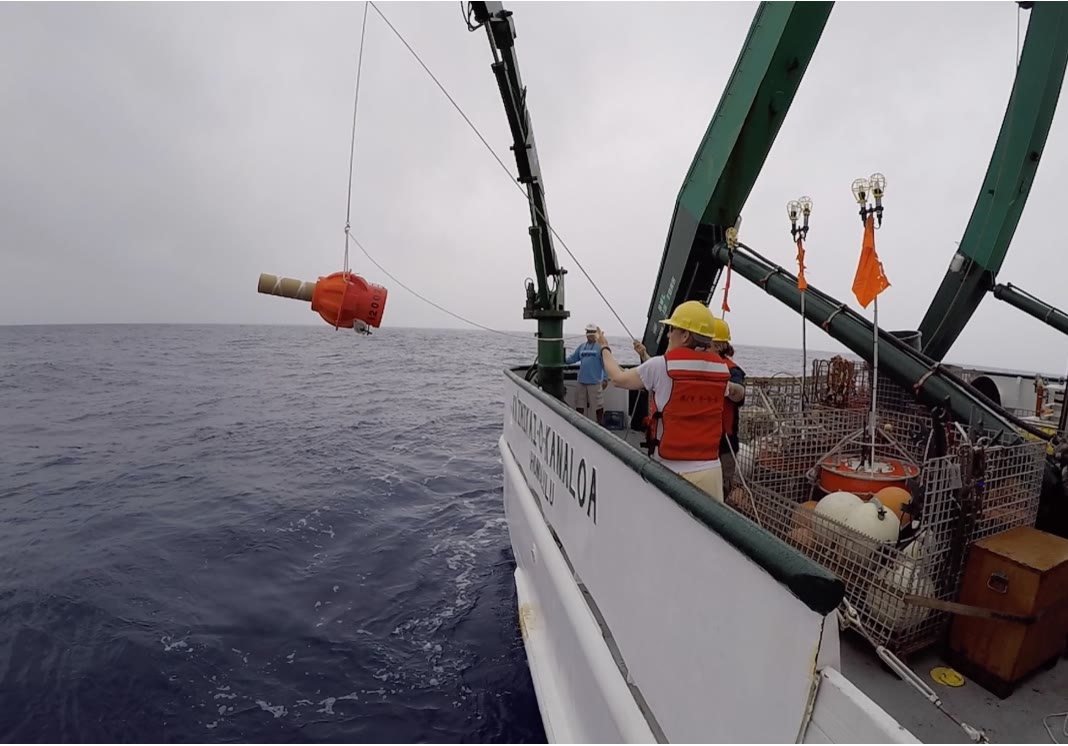
\includegraphics[width=0.6\linewidth]{images/book3/b1-deep-float.jpg}

{\small Pelampung profil samudra dalam (instrumen oranye yang tergantung dari derek) diturunkan dari kapal riset pada 2018; setelah dilepaskan, ia tenggelam ke kedalaman kerjanya dan naik ke permukaan pada selang teratur untuk mengirim datanya. (Fotografer NOAA yang tidak diketahui, domain publik, melalui Wikimedia Commons.)}
\label{fig:b1:ocean-circulation:float}
\end{omfigure}
% ledger: commons:deep-solo, noaa:argo-25

Pembalikan membawa panas. Air yang pergi ke utara dalam keadaan hangat dan kembali dalam keadaan dingin telah melepaskan panas kepada atmosfer di utara.

\begin{proposition}[Panas yang dibawa oleh pembalikan]\label{prop:b1:ocean-circulation:heat}
Jika transpor volume $Q$ melintasi suatu \omterm{def:b1:spherical-astronomy:geographic}{lintang} ke utara pada \omterm{def:b1:fluid-envelopes-structure:potential-temperature}{suhu potensial} $\theta_1$ dan kembali ke selatan pada $\theta_2$, tanpa transpor massa neto, pembalikan itu membawa ke utara fluks panas
\[
  H = \rho c_p\,Q\,(\theta_1 - \theta_2),
\]
dengan $c_p$ adalah kalor jenis air laut.
\end{proposition}
% ledger: teos10:cp0

\begin{proof}
Setiap detik, massa $\rho Q$ melintas ke utara membawa kandungan panas $\rho Q
c_p\theta_1$, dihitung dari nol suhu yang sembarang, dan massa yang sama melintas ke selatan membawa $\rho Q c_p\theta_2$. Fluks neto ke utara adalah selisihnya; karena kedua massa sama, nol yang sembarang itu saling meniadakan, dan hasilnya adalah transpor panas yang sungguhan.
\end{proof}

Anggaran kasar Atlantik Utara, oleh W.~Schmitz, memiliki Arus Teluk membawa \qty{40}{\sverdrup} air pada \qty{18}{\celsius} ke utara, dari jumlah itu
\qty{14}{\sverdrup} kembali ke selatan sebagai air dalam pada \qty{2}{\celsius}. Dengan $c_p =
\qty{3992}{J.kg^{-1}.K^{-1}}$ dan $\rho = \qty{1027}{kg.m^{-3}}$, pembalikan ini membawa $1027 \times 3992 \times \num{14e6} \times 16 = \qty{0.92e15}{W}$, sekitar \qty{0.9}{PW}, ke utara \ang{24} LU; estimasi yang cermat memberi \qty{1.2}{PW}, seperempat transpor panas ke arah kutub oleh atmosfer dan samudra bersama. Sebagian besar panas ini diberikan kepada udara di atas Atlantik Utara bagian utara, yang merupakan salah satu alasan mengapa Norwegia, pada \ang{60} LU, jauh lebih hangat daripada Greenland selatan pada \omterm{def:b1:spherical-astronomy:geographic}{lintang} yang sama.
% ledger: stewart:heat-conveyor, rapid:home, teos10:cp0 (computed in calc/ch29.py)

Sirkulasi dalam lambat. Jika butuh sekitar seribu tahun bagi air yang tenggelam di Atlantik Utara untuk mencapai Pasifik Utara melalui Arus Sirkumpolar Antartika, kelajuan rerata-nya sekitar \qty{1}{mm/s}, seratus kali lebih lambat daripada arus dalam yang bervariasi yang dicatat pengukur arus. Kelajuannya karena itu disimpulkan dari traser alih-alih diukur: tritium, yang dilepaskan ke atmosfer oleh uji nuklir 1950-an dan meluruh dengan waktu paruh \qty{12.3}{tahun}, memasuki Atlantik Utara dalam tempat air dalam terbentuk, dan setelah 25 tahun telah menyebar sedikit ke selatan \ang{30} LU, kelajuan rerata kurang dari \qty{1}{mm/s}. Volume samudra dibagi dengan laju \omterm{def:b1:ocean-circulation:moc}{pembentukan air dalam} memberi skala waktu yang sama (\cref{exo:b1:ocean-circulation:12}).
% ledger: stewart:deep-circulation, nos:conveyor

Arus Sirkumpolar Antartika menghubungkan cekungan-cekungan. Arusnya mencapai dasar laut dan lambat, sekitar \qty{10}{cm/s}, hingga \qty{50}{cm/s} di frontnya, tetapi ia dalam dan lebar: deretan pengukur arus tertambat melintasi Selat Drake, antara Amerika Selatan dan Antartika, memberi \qty[uncertainty-mode=separate]{125 \pm 11}{\sverdrup} (diterbitkan pada 1985), dan deretan yang lebih rapat pada 2007--2011, yang juga mengukur arus dekat dasar, memberi \qty{173.3}{\sverdrup}, \qty{39}{\percent} lebih banyak daripada nilai lama yang dipakai itu. Ia membawa air dalam dari setiap samudra ke samudra lain dan mencampurnya di sepanjang jalan.
% ledger: stewart:acc, donohue:acc

\begin{dated}{2021}
% ledger: ipcc:amoc-observed, ipcc:amoc-projected
Penilaian 2021 Panel Antarpemerintah tentang Perubahan Iklim (IPCC) menyimpulkan, dari rekonstruksi, bahwa pembalikan Atlantik relatif stabil sepanjang \num{8000} tahun terakhir (\emph{keyakinan sedang}), dengan pelemahan yang mulai pada akhir abad ke-19 (\emph{keyakinan sedang}), tetapi hanya memiliki \emph{keyakinan rendah} pada penurunan menyeluruh selama abad ke-20. Pelemahan yang diamati langsung dari pertengahan 2000-an hingga pertengahan 2010-an (\emph{keyakinan tinggi}) tidak dapat dibedakan dari variabilitas skala dasawarsa (\emph{keyakinan tinggi}). Pembalikan \emph{sangat mungkin} melemah sepanjang abad ke-21 untuk semua skenario emisi, dengan hanya \emph{keyakinan rendah} pada besarnya penurunan itu; ada \emph{keyakinan sedang} bahwa ia tidak akan runtuh secara mendadak sebelum 2100.
\end{dated}

\section{Latihan}

\begin{exercise}[$\star$]\label{exo:b1:ocean-circulation:1}
Gunakan rumus massal dengan $\rho_a = \qty{1.3}{kg.m^{-3}}$ dan koefisien seret Yelland dan Taylor. (a)~Hitung $C_D$ dan \omterm{def:b1:ocean-circulation:wind-stress}{tegangan angin} untuk angin \qty{4}{m/s}, \qty{7}{m/s} dan \qty{15}{m/s}. (b)~Dengan faktor berapa tegangan tumbuh dari 7 ke \qty{15}{m/s}? Bandingkan dengan rasio kuadrat kelajuannya dan jelaskan selisihnya.
% ledger: stewart:wind-stress, stewart:drag-coefficient
\end{exercise}

\begin{exercise}[$\star$]\label{exo:b1:ocean-circulation:2}
Berikan arah \omterm{def:b1:ocean-circulation:ekman}{transpor Ekman} pada setiap kasus. (a)~Angin yang berhembus ke timur pada \ang{45} LU. (b)~\omterm{def:b1:atmospheric-circulation:winds}{Angin pasat} dari timur laut pada \ang{15} LU. (c)~Angin yang berhembus ke timur pada \ang{50} LS. (d)~Angin dari selatan sepanjang pantai barat Afrika selatan, dekat \ang{23} LS. Pada manakah dari keempat kasus transpor menunjuk ke lepas pantai, dan apa yang mengikutinya?
\end{exercise}

\begin{exercise}[$\star$]\label{exo:b1:ocean-circulation:3}
Pada \ang{26.5} LU di Atlantik, transpor rerata 2004--2024 adalah: Selat Florida \qty{31.7}{\sverdrup}, Ekman \qty{3.5}{\sverdrup}, tengah samudra atas \qty{-17.9}{\sverdrup}; menurut lapisan, 0--\qty{800}{m} \qty{16.6}{\sverdrup}, 800--\qty{1100}{m} \qty{0.4}{\sverdrup}, 1100--\qty{3000}{m} \qty{-12.0}{\sverdrup}, 3000--\qty{5000}{m} \qty{-5.9}{\sverdrup} (ke utara positif). (a)~Jumlahkan tiga yang pertama dan bandingkan dengan pembalikan yang diterbitkan, \qty{17.1}{\sverdrup}. (b)~Bandingkan aliran ke utara di atas \qty{1100}{m} dengan aliran ke selatan di bawahnya. (c)~Konversikan \qty{17.1}{\sverdrup} menjadi kilometer kubik per tahun, dan hitung waktu yang dibutuhkan aliran ini untuk mengisi volume seluruh samudra, \qty{1.3324e9}{km^3}.
% ledger: rapid:transports, charette:ocean-volume
\end{exercise}

\begin{exercise}[$\star$]\label{exo:b1:ocean-circulation:4}
Dengan rumus Ekman, hitung kedalaman Ekman dan arus permukaan di bawah angin \qty{10}{m/s} pada \ang{15}, \ang{45} dan \ang{60} \omterm{def:b1:spherical-astronomy:geographic}{lintang}, serta arus permukaan sebagai persentase angin. Mengapa rumusnya gagal dekat khatulistiwa?
% ledger: stewart:ekman-constants
\end{exercise}

\begin{exercise}[$\star\star$]\label{exo:b1:ocean-circulation:5}
Di \ang{11} LU di Atlantik, ambil \omterm{def:b1:ocean-circulation:wind-stress}{tegangan angin} rerata \qty{0.07}{Pa} ke barat melintasi lebar \qty{5000}{km}, dan $\rho = \qty{1027}{kg.m^{-3}}$. (a)~Hitung \omterm{def:b1:ocean-circulation:ekman}{transpor Ekman} per meter dan arahnya. (b)~Hitung transpor volume total melintasi irisan dalam \omterm{def:b1:ocean-circulation:ekman}{sverdrup}. (c)~Bandingkan dengan transpor yang diukur langsung ($12.0 \pm \qty{5.5}{\sverdrup}$) dan yang dihitung dari angin jangka panjang ($13.5 \pm \qty{0.3}{\sverdrup}$).
% ledger: stewart:ekman-transport
\end{exercise}

\begin{exercise}[$\star\star$]\label{exo:b1:ocean-circulation:6}
Di sepanjang Pasifik khatulistiwa, \omterm{def:b1:atmospheric-circulation:winds}{angin pasat} memberikan tegangan \qty{0.05}{Pa} ke barat. (a)~Hitung \omterm{def:b1:ocean-circulation:ekman}{transpor Ekman} per meter, dan arahnya, pada \ang{2} LU dan pada \ang{2}~LS. (b)~Dengan menganggap bahwa air yang dibawa pergi melintasi kedua \omterm{def:b1:spherical-astronomy:geographic}{lintang} ini diganti dari bawah di antara keduanya, hitung kecepatan \omterm{def:b1:ocean-circulation:upwelling}{upwelling} rerata dalam meter per hari. (c)~Apa yang terjadi dengan rumus teorema tepat di khatulistiwa? Kesimpulan mana yang tetap berlaku?
\end{exercise}

\begin{exercise}[$\star\star$]\label{exo:b1:ocean-circulation:7}
Di atas \omterm{def:b1:ocean-circulation:gyre}{gyre subtropik}, ambil \omterm{def:b1:ocean-circulation:wind-stress}{tegangan angin} \qty{0.06}{Pa} ke barat pada \ang{15} LU dan \qty{0.12}{Pa} ke timur pada \ang{40} LU. (a)~Hitung kedua \omterm{def:b1:ocean-circulation:ekman}{transpor Ekman} dan arahnya. (b)~Dengan menganggap transpor berubah seragam di antara kedua \omterm{def:b1:spherical-astronomy:geographic}{lintang}, hitung kecepatan vertikal di dasar \omterm{def:b1:ocean-circulation:ekman}{lapisan Ekman}, dalam meter per tahun, dan katakan apakah ke atas atau ke bawah. (c)~Di atas cekungan selebar \qty{5000}{km}, berapa \omterm{def:b1:ocean-circulation:ekman}{sverdrup} yang dipompa melalui dasar lapisan?
\end{exercise}

\begin{exercise}[$\star\star$]\label{exo:b1:ocean-circulation:8}
Ambil $\rho = \qty{1027}{kg.m^{-3}}$ dan $c_p = \qty{3992}{J.kg^{-1}.K^{-1}}$. (a)~Hitung panas yang dibawa ke utara oleh \qty{17}{\sverdrup} yang mengalir ke utara pada \qty{15}{\celsius} dan kembali pada \qty{3}{\celsius}. (b)~Bandingkan dengan \qty{1.2}{PW} yang dibawa oleh pembalikan Atlantik. (c)~Jika air yang sama kembali ke selatan di permukaan, di sepanjang sisi timur cekungan, pada \qty{12}{\celsius}, panas apa yang akan dibawanya? Apa yang dikatakan ini tentang pentingnya \omterm{def:b1:ocean-circulation:moc}{pembentukan air dalam}?
% ledger: rapid:home, teos10:cp0
\end{exercise}

\begin{exercise}[$\star\star$]\label{exo:b1:ocean-circulation:9}
Tiga \omterm{def:b1:fluid-envelopes-structure:ts-diagram}{massa air} Atlantik Selatan memiliki \omterm{def:b1:fluid-envelopes-structure:potential-temperature}{suhu potensial} dan salinitas: Air Menengah Antartika \qty{3.3}{\celsius}, 34.15; Air Dalam Atlantik Utara \qty{4.0}{\celsius}, 35.00; Air Dasar Antartika \qty{0.4}{\celsius}, 34.67. Sebuah sampel pada kedalaman memiliki $\theta = \qty{2.78}{\celsius}$ dan $S = 34.731$. Dengan \cref{prop:b1:fluid-envelopes-structure:mixing}, temukan bagian setiap \omterm{def:b1:fluid-envelopes-structure:ts-diagram}{massa air} dalam sampel.
% ledger: stewart:deep-circulation
\end{exercise}

\begin{exercise}[$\star\star\star$]\label{exo:b1:ocean-circulation:10}
Ambil spiral \cref{prop:b1:ocean-circulation:spiral}. (a)~Tunjukkan bahwa $u$ dan $v$
memenuhi $f v + A_z u'' = 0$ dan $-f u + A_z v'' = 0$. (Petunjuk: tulis $u + iv =
V_0\,e^{i\pi/4}\,e^{(1+i)az}$.) (b)~Tunjukkan bahwa tegangan $\rho A_z\,\partial\vec
v/\partial z$ di permukaan sama dengan \omterm{def:b1:ocean-circulation:wind-stress}{tegangan angin} $(0, T)$. (c)~Hitung transpor $\int_{-\infty}^0 \rho u\,\mathrm dz$ dan $\int_{-\infty}^0 \rho
v\,\mathrm dz$, dan periksa bahwa keduanya sesuai dengan
\cref{thm:b1:ocean-circulation:ekman}.
\end{exercise}

\begin{exercise}[$\star\star\star$]\label{exo:b1:ocean-circulation:11}
Dalam model Stommel, \omterm{def:b1:ocean-circulation:wbc}{arus batas barat} memiliki lebar sekitar $R/\beta$, dengan $R$ laju gesekan dasar dan $\beta = \mathrm df/\mathrm dy$ laju kenaikan \omterm{def:b1:atmospheric-circulation:coriolis-parameter}{parameter Coriolis} ke utara. (a)~Tunjukkan bahwa $\beta = 2\Omega
\cos\varphi/a_\oplus$ dan hitung pada \ang{30} LU ($a_\oplus = \qty{6371}{km}$). (b)~Dengan $R = \qty{e-6}{s^{-1}}$, hitung lebarnya. (c)~Transpor \qty{30}{\sverdrup} hanyut ke selatan melintasi interior cekungan selebar \qty{5000}{km} dalam \qty{1000}{m} atas, dan kembali ke utara dalam arus batas pada kedalaman yang sama. Hitung kedua kelajuan rerata dan bandingkan dengan kelajuan Arus Teluk, \qty{1.8}{m/s}.
% ledger: stewart:north-atlantic, nos:gulf-stream, earth:Rmean
\end{exercise}

\begin{exercise}[$\star\star\star$]\label{exo:b1:ocean-circulation:12}
Samudra menampung \qty{1.3324e9}{km^3} di atas \qty{361.84e6}{km^2}. (a)~Tunjukkan bahwa volume di bawah \qty{1000}{m} setidaknya \qty{9.71e8}{km^3}. (b)~Air Dalam Atlantik Utara terbentuk sekitar \qty{17}{\sverdrup} dan Air Dasar Antartika sekitar \qty{9}{\sverdrup}. Perkirakan waktu yang dibutuhkan untuk memperbarui air di bawah \qty{1000}{m}, dan bandingkan dengan seribu tahun konveyor. (c)~Tritium memiliki waktu paruh \qty{12.3}{tahun}. Berapa bagian masukan tritium yang tersisa setelah 25 tahun? Seberapa jauh air yang bergerak dengan \qty{1}{mm/s} menempuh dalam 25 tahun?
% ledger: charette:ocean-volume, stewart:deep-circulation, stewart:acc, rapid:transports
\end{exercise}

\section{Masalah: pantai upwelling}

\begin{problem}[{Soal akhir pekan --- angin musim panas sepanjang pantai pada \ang{38} LU}]
\label{pb:b1:ocean-circulation:1}
% nilai: calc/ch29.py (pantai fiktif; konstanta dari ledger)
Sebuah pantai lurus membentang utara--selatan pada \ang{38} LU, dengan samudra di barat. Pada musim panas, angin mantap \qty{8}{m/s} berhembus dari utara sepanjang pantai selama berminggu-minggu. Pantai itu fiktif, tetapi angkanya khas bagi sisi timur samudra. Gunakan $\Omega = 2\pi/(\qty{23.9345}{h})$, $\rho_a = \qty{1.3}{kg.m^{-3}}$, koefisien seret Yelland dan Taylor, $\rho = \qty{1027}{kg.m^{-3}}$ untuk air laut dan $c_p = \qty{3992}{J.kg^{-1}.K^{-1}}$.

\medskip
\noindent\textbf{Bagian I --- Angin dan tegangannya.}
\begin{enumerate}
  \item Ke arah mana angin berhembus? Apakah sejajar dengan pantai atau melintasinya?
  \item Hitung koefisien seret.
  \item Hitung \omterm{def:b1:ocean-circulation:wind-stress}{tegangan angin}.
  \item Pertanyaan yang sama untuk angin \qty{12}{m/s}. Dengan faktor berapa tegangan tumbuh, dan mengapa lebih besar daripada rasio kuadrat kelajuan?
  \item Hitung \omterm{def:b1:atmospheric-circulation:coriolis-parameter}{parameter Coriolis} pada \ang{38} LU.
  \item Hitung $2\pi/f$ dalam jam. Mengapa angin harus berhembus selama sehari atau lebih sebelum keseimbangan Ekman berlaku?
\end{enumerate}

\medskip
\noindent\textbf{Bagian II --- Lapisan Ekman.}
\begin{enumerate}[resume]
  \item Ke arah mana transpor massa Ekman? Ke arah daratan atau laut lepas?
  \item Hitung transpor massa Ekman per meter pantai.
  \item Konversikan menjadi transpor volume per meter.
  \item Hitung kedalaman Ekman dengan rumus Ekman.
  \item Hitung rerata kecepatan lepas pantai dalam lapisan, dalam \unit{cm/s}.
  \item Hitung arus permukaan dengan rumus Ekman, dan arahnya. Apa yang diberikan pengukuran pelampung untuk kelajuannya?
\end{enumerate}

\medskip
\noindent\textbf{Bagian III --- Upwelling di pantai.}
\begin{enumerate}[resume]
  \item Jelaskan, dengan sketsa irisan vertikal, dari mana asal air yang dibawa ke lepas pantai.
  \item Hitung volume yang di-upwell per hari di sepanjang setiap kilometer pantai.
  \item Anggaplah air naik melalui pita selebar \qty{20}{km} di sepanjang pantai. Hitung kecepatan naik rerata, dalam \unit{m/s} dan dalam meter per hari.
  \item Berapa lama air membutuhkan waktu untuk naik dari dasar \omterm{def:b1:ocean-circulation:ekman}{lapisan Ekman} ke permukaan dengan kelajuan ini?
  \item Air yang di-upwell mencapai permukaan pada \qty{12}{\celsius}, sedangkan laut terbuka di lepas pantai berada pada \qty{18}{\celsius}. Angin laut membawa udara hangat dan lembap dari lepas pantai di atas air ini. Apa yang terjadi pada udara dekat permukaan, dan cuaca apa yang mengikutinya di pantai?
  \item Mengapa pantai seperti itu kaya ikan?
  \item Pada musim gugur angin berbalik dan berhembus dari selatan selama seminggu. Apa yang terjadi pada transpor dan pada air di pantai?
\end{enumerate}

\medskip
\noindent\textbf{Bagian IV --- Pantai lain dan transpor total.}
\begin{enumerate}[resume]
  \item Dengan tegangan yang sama, hitung \omterm{def:b1:ocean-circulation:ekman}{transpor Ekman} per meter pada \ang{20} LU dan bandingkan dengan \ang{38} LU.
  \item Di pantai barat Afrika selatan, dekat \ang{23} LS, arah angin mana yang menggerakkan \omterm{def:b1:ocean-circulation:upwelling}{upwelling}? Bandingkan dengan pantai soal ini.
  \item Di bawah angin \qty{5}{m/s} alih-alih \qty{8}{m/s} pada \ang{38} LU, hitung tegangan dan \omterm{def:b1:ocean-circulation:ekman}{transpor Ekman} per meter, dan rasionya terhadap yang ada pada soal~8.
  \item Air yang di-upwell menghangat \qty{6}{\celsius} saat menyimpang ke lepas pantai. Hitung panas yang diserapnya per detik per meter pantai, lalu sepanjang \qty{1000}{km}.
  \item Berapa panjang pantai seperti itu yang akan meng-upwell air sebanyak yang dibawa Arus Teluk melalui Selat Florida, \qty{31.7}{\sverdrup}?
  \item Berapa volume air, dalam \omterm{def:b1:ocean-circulation:ekman}{sverdrup}, yang di-upwell sepanjang \qty{1000}{km} pantai ini?
\end{enumerate}
\end{problem}
